\subsection{Package della componente Model}
	\begin{figure}[h!]
	\begin{center}
		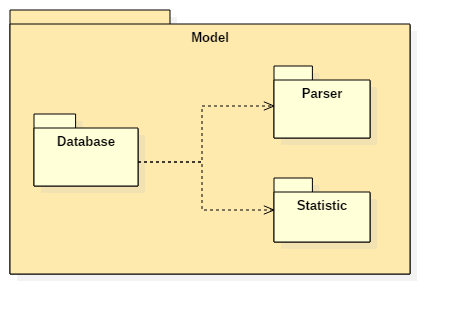
\includegraphics[scale=0.65]{../images/ModelPackage.png}
		\caption{Package della componente Model}
	\end{center}
	\end{figure}
	Il package per il componente Model del pattern architetturale MVP contiene i seguenti sotto packages:
	\begin{itemize}
		\item\textbf{Database:} questo package si occuperà di gestire le richieste in arrivo dal Presenter e avviserà quest'ultimo ogni qualvolta si verifica un cambiamento dei dati salvati nel sistema tramite appositi eventi; Per fare ciò si avvale delle classi:
			\begin{itemize}
				\item\textit{Database}
				\item\textit{QuestionModifiedEvent}
				\item\textit{QuestionRemovedEvent}
				\item\textit{QuizModifiedEvent}
				\item\textit{QuizRemovedEvent}
				\item\textit{UserCreatedEvent}
				\item\textit{UserModifiedEvent}
				\item\textit{UserRemovedEvent}
			\end{itemize}
				e delle seguenti interfacce:
			\begin{itemize}
				\item\textit{ModelEvent}
			\end{itemize}
		\item\textbf{Parser:} questo package fornisce funzionalità per il controllo sintattico rispetto a QML; Per fare ciò si avvale delle classi:
			\begin{itemize}
				\item\textit{Parser}
			\end{itemize}
		\item\textbf{Statistic:} questo package fornisce classi per il raccoglimento delle statistiche relative ai quesiti, questionari ed utenti; Per fare ciò si avvale delle classi:
			\begin{itemize}
				\item\textit{Statistics}
			\end{itemize}
		\end{itemize}
		\newpage